% \documentclass[aspectratio=169, 11pt]{beamer}
\documentclass[aspectratio=169, 11pt, handout]{beamer}

% ── Theme ──
\usetheme{Madrid}
\usecolortheme{default}
\setbeamertemplate{navigation symbols}{}
\setbeamertemplate{footline}{%
  \leavevmode\hbox{%
    \begin{beamercolorbox}[wd=.333333\paperwidth,ht=2.5ex,dp=1ex,center]{author in head/foot}%
      \usebeamerfont{author in head/foot}\insertshortauthor
    \end{beamercolorbox}%
    \begin{beamercolorbox}[wd=.333333\paperwidth,ht=2.5ex,dp=1ex,center]{title in head/foot}%
      \usebeamerfont{title in head/foot}\insertshorttitle
    \end{beamercolorbox}%
    \begin{beamercolorbox}[wd=.333333\paperwidth,ht=2.5ex,dp=1ex,right]{date in head/foot}%
      \usebeamerfont{date in head/foot}\insertframenumber{} / \inserttotalframenumber\hspace*{2ex}
    \end{beamercolorbox}}}

% ── Packages ──
\usepackage{amsmath,amssymb}
\usepackage{booktabs}
\usepackage{xcolor}
\usepackage{colortbl}
\usepackage{tikz}
\usetikzlibrary{arrows.meta, positioning}
\usetikzlibrary{calc}

% ── Colors ──
\definecolor{sbgreen}{HTML}{00704A}
\definecolor{abnbred}{HTML}{FF5A5F}
\definecolor{warnred}{HTML}{CC0000}
\definecolor{noteblue}{HTML}{2060A0}

% ── Commands ──
\newcommand{\E}{\mathbb{E}}
\newcommand{\Var}{\mathrm{Var}}
\newcommand{\Cov}{\mathrm{Cov}}
\newcommand{\SE}{\mathrm{SE}}
\newcommand{\Prob}{\mathrm{Pr}}
\newcommand{\indep}{\perp\!\!\!\perp}
\DeclareMathOperator{\plim}{plim}

% ── Reusable TikZ styles ──
\tikzset{
    tnode/.style={draw, rounded corners, fill=gray!10, minimum width=2.2cm, minimum height=0.65cm, font=\small, align=center},
    tgreen/.style={tnode, fill=sbgreen!15, draw=sbgreen},
    tblue/.style={tnode, fill=noteblue!12, draw=noteblue},
    tred/.style={tnode, fill=abnbred!15, draw=abnbred},
    twarn/.style={tnode, fill=red!8, draw=warnred},
    tarrow/.style={-{Stealth}, thick}
}

% ── Title ──
\title[Lecture 8]{Lecture 8: Double Machine Learning}
\subtitle{Applied ML for Business Part II}
\author{Zhikun Lu}
\date{\today}

\begin{document}

% ====================================================================
\begin{frame}
\titlepage
\end{frame}

% ====================================================================
\begin{frame}{Where We Are}

\begin{center}
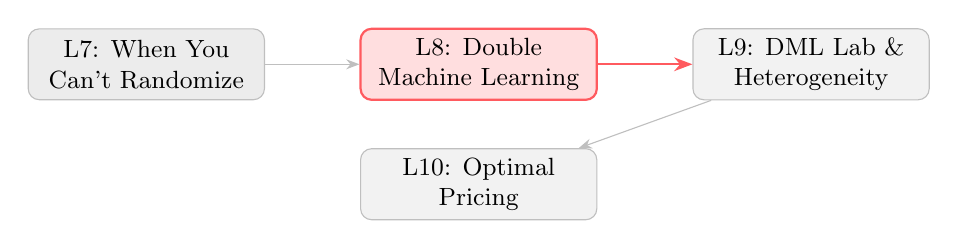
\begin{tikzpicture}[
    node distance=0.6cm and 1.2cm,
    box/.style={draw, rounded corners, minimum width=3cm, minimum height=0.9cm, font=\small, align=center},
    done/.style={box, fill=gray!15, draw=gray!50},
    active/.style={box, fill=abnbred!20, draw=abnbred, thick},
    inactive/.style={box, fill=gray!10, draw=gray!50}
]
\node[done]               (L7)  {L7: When You\\Can't Randomize};
\node[active, right=of L7](L8)  {L8: Double\\Machine Learning};
\node[inactive, right=of L8](L9){L9: DML Lab \&\\Heterogeneity};
\node[inactive, below=of L8](L10){L10: Optimal\\Pricing};

\draw[-{Stealth}, gray!50]        (L7) -- (L8);
\draw[-{Stealth}, thick, abnbred] (L8) -- (L9);
\draw[-{Stealth}, gray!50]        (L9) -- (L10);
\end{tikzpicture}
\end{center}

\bigskip

\textbf{Last time:} the PLR model $Y = \theta D + g(X) + \varepsilon$ separates the causal parameter $\theta$ from the nuisance $g(X)$. But OLS cannot capture nonlinear $g$, and Lasso regularizes $\theta$ along with everything else.

\bigskip

\textbf{Today:} DML uses ML to handle the nuisance without letting ML error contaminate $\hat{\theta}$.

\end{frame}

% ====================================================================
\begin{frame}{Today's Plan}

\begin{enumerate}
    \item \textbf{The naive plugin.} Estimate $g(X)$ with ML, plug in, and why it fails
    \item \textbf{Reducing the bias.} Remove the predictable part of $D$
    \item \textbf{Why the fix works.} The bias becomes a product of two errors
    \item \textbf{Cross-fitting.} Handling overfitting bias
    \item \textbf{From theory to practice.} The FWL connection and the DML algorithm
    \item \textbf{The general principle.} Beyond PLR
\end{enumerate}

\end{frame}


% %%%%%%%%%%%%%%%%%%%%%%%%%%%%%%%%%%%%%%%%%%%%%%%%%%%%%%%%%%%%%%%%%%%%
% ACT 1: THEORY (g/m formulation)
% %%%%%%%%%%%%%%%%%%%%%%%%%%%%%%%%%%%%%%%%%%%%%%%%%%%%%%%%%%%%%%%%%%%%

% %%%%%%%%%%%%%%%%%%%%%%%%%%%%%%%%%%%%%%%%%%%%%%%%%%%%%%%%%%%%%%%%%%%%
\section{The Naive Plugin}
% %%%%%%%%%%%%%%%%%%%%%%%%%%%%%%%%%%%%%%%%%%%%%%%%%%%%%%%%%%%%%%%%%%%%

% ====================================================================
\begin{frame}{Recap: The Partially Linear Model}

From L7, the estimation problem:

\begin{block}{Partially Linear Model (Robinson 1988)}
\[
Y_i = \theta D_i + g(X_i) + \varepsilon_i, \qquad \E[\varepsilon_i \mid D_i, X_i] = 0
\]
\end{block}

The confounding structure: $D_i$ depends on $X_i$ through $r(X_i) = \E[D_i \mid X_i]$.

\bigskip

\begin{tabular}{ll}
$\theta$ & price elasticity (target) \\
$g(X)$ & listing quality effect (nuisance) \\
$r(X) = \E[D \mid X]$ & confounding: how $X$ affects pricing \\
\end{tabular}

\bigskip
\pause

The challenge: $g(X)$ is an unknown nonlinear function of 80+ features. We cannot estimate it with OLS, and Lasso regularizes $\theta$ along with everything else.

\end{frame}

% ====================================================================
\begin{frame}{The Natural Moment Condition}

If we knew $g$, estimation would be straightforward. From $Y - g(X) = \theta D + \varepsilon$, we directly regress $Y - g(X)$ on $D$, using the following moment condition (FOC from min MSE):

\[
\E\bigl[D_i \cdot (Y_i - \theta D_i - g(X_i))\bigr] = 0
\]

\pause
\bigskip

Solving for $\theta$:
\[
\theta = \frac{\E[D_i(Y_i - g(X_i))]}{\E[D_i^2]}
\]

\pause
\bigskip

\textbf{The plugin idea:} we don't know $g$, but suppose we can estimate it with ML. Call the estimate $\hat{g}$. Plug it in:

\[
\hat{\theta}_{\text{naive}} = \frac{\sum_i D_i(Y_i - \hat{g}(X_i))}{\sum_i D_i^2}
\]

\end{frame}



% ====================================================================
\begin{frame}{The Plugin Bias}

Substitute $Y_i = \theta_0 D_i + g(X_i) + \varepsilon_i$:

\[
\hat{\theta}_{\text{naive}} - \theta_0 = \underbrace{\frac{\sum_i D_i \varepsilon_i}{\sum_i D_i^2}}_{\text{sampling noise}} + \underbrace{\frac{\sum_i D_i\bigl(g(X_i) - \hat{g}(X_i)\bigr)}{\sum_i D_i^2}}_{\text{plugin bias}}
\]

\pause
\bigskip

The first term is standard sampling noise: $O_p(n^{-1/2})$ by the CLT.

\bigskip

The second term is estimation error from $\hat{g}$: generally $O(\|\hat{g} - g\|)$.

\bigskip

How fast does $\hat{g}$ converge?

\end{frame}


% ====================================================================
\begin{frame}{The Regularization Bias}

\[
\sqrt{n}(\hat{\theta}_{\text{naive}} - \theta_0) = \underbrace{\frac{\frac{1}{\sqrt{n}}\sum_i D_i \varepsilon_i}{\frac{1}{n}\sum_i D_i^2}}_{\to\; N(0, V)} \;+\; \underbrace{\sqrt{n} \cdot O\bigl(\|\hat{g} - g\|\bigr)}_{\text{regularization bias}}
\]

\pause

ML methods (lasso, forests, neural nets) achieve flexibility through \textbf{regularization}, which trades bias for variance. This is the same regularization that biased $\hat{\theta}$ directly in L7; at the high level, it limits the convergence rate of $\hat{g}$:

\[
\|\hat{g} - g\| = O(n^{-s}) \quad \text{where } s < \tfrac{1}{2} \text{ (typically } s > \tfrac{1}{4}\text{)}
\]

\pause

So the bias term grows: $\sqrt{n} \cdot o(n^{-1/4}) = o(n^{1/4})$ could explode.

\bigskip

\textbf{Result:} $\hat{\theta}_{\text{naive}}$ is not $\sqrt{n}$-consistent. Standard inference is invalid.

\end{frame}


% %%%%%%%%%%%%%%%%%%%%%%%%%%%%%%%%%%%%%%%%%%%%%%%%%%%%%%%%%%%%%%%%%%%%
\section{Reducing the Bias}
% %%%%%%%%%%%%%%%%%%%%%%%%%%%%%%%%%%%%%%%%%%%%%%%%%%%%%%%%%%%%%%%%%%%%

\begin{frame}{Locating the Bias}

Where inside $D_i$ does the plugin bias come from? Let $r(X) = \mathbb{E}[D \mid X]$ and split $D_i$ into its predictable and unpredictable parts:
\[
D_i = \underbrace{r(X_i)}_{\text{predictable}} + \underbrace{\tilde{D}_i}_{\tilde{D}_i := D_i - r(X_i)}
\]

This gives the decomposition:
\[
\frac{1}{n}\sum_i D_i(g - \hat{g})(X_i)
=
\underbrace{\frac{1}{n}\sum_i r(X_i)(g - \hat{g})(X_i)}_{\text{(A) predictable part}}
+
\underbrace{\frac{1}{n}\sum_i \tilde{D}_i(g - \hat{g})(X_i)}_{\text{(B) unpredictable part}}
\]

\pause
\bigskip

\textbf{(A) Predictable part: first-order bias.}

\[
\left| \mathbb{E}[r(X)(g - \hat{g})(X)] \right|
\le \|r\|_2 \cdot \|\hat{g} - g\|_2
\]

This term is $O_p(\|\hat{g} - g\|)$: it directly inherits the slow convergence rate of ML.

\end{frame}




\begin{frame}{Locating the Bias (cont.)}

\textbf{(B) Unpredictable part: why it's harmless.}

Treat $\hat{g}$ as fixed (imagine it was trained on a separate, independent sample). Then, since $\mathbb{E}[\tilde{D}_i \mid X_i] = 0$ by construction:
\[
\mathbb{E}\!\left[\tilde{D}_i (g - \hat{g})(X_i) \;\big|\; \hat{g}\right]
= \mathbb{E}\!\left[(g - \hat{g})(X_i) \cdot \underbrace{\mathbb{E}[\tilde{D}_i \mid X_i]}_{=\,0}\right] = 0.
\]

\pause

So the summands are i.i.d.\ mean zero, each of size $O_p(\|\hat{g} - g\|)$. A CLT gives:
\[
\frac{1}{n}\sum_i \tilde{D}_i(g - \hat{g})(X_i) = O_p\!\left(\frac{\|\hat{g} - g\|}{\sqrt{n}}\right)
\]

This is negligible compared to (A). \emph{(We will revisit the ``$\hat{g}$ fixed'' assumption shortly.)}

\end{frame}


\begin{frame}{Diagnosis and Prescription}

\textbf{Diagnosis.} The first-order bias lives entirely in A, the predictable part of $D$. The unpredictable part $\tilde{D}$ is already harmless.

\pause
\bigskip

\textbf{Prescription.} Build a new moment condition around $\tilde{D}$ instead of $D$:
\[
\mathbb{E}\bigl[\tilde{D}\,(Y - g(X) - \theta D)\bigr] = 0
\]
The plugin bias from $\hat{g}$ becomes the harmless term B, by construction.

\pause
\bigskip

\textbf{But} $\tilde{D}_i = D_i - r(X_i)$ is not observable: we don't know $r$.

\end{frame}


% %%%%%%%%%%%%%%%%%%%%%%%%%%%%%%%%%%%%%%%%%%%%%%%%%%%%%%%%%%%%%%%%%%%%
\section{Why the Fix Works}
% %%%%%%%%%%%%%%%%%%%%%%%%%%%%%%%%%%%%%%%%%%%%%%%%%%%%%%%%%%%%%%%%%%%%

% ====================================================================
\begin{frame}{From One Error to Two}

So estimate $r$ too. Using $\hat{r}$ in place of $r$:
\[
\hat{\tilde{D}}_i = D_i - \hat{r}(X_i) = \tilde{D}_i + (r - \hat{r})(X_i)
\]

The plugin bias in the new moment condition becomes:
\[
\frac{1}{n}\sum_i \hat{\tilde{D}}_i (g - \hat{g})(X_i)
=
\underbrace{\frac{1}{n}\sum_i \tilde{D}_i (g - \hat{g})(X_i)}_{\text{harmless (term B)}}
+
\underbrace{\frac{1}{n}\sum_i (r - \hat{r})(X_i)(g - \hat{g})(X_i)}_{\text{cost of not knowing } r}
\]

\pause
\bigskip

We have traded a single first-order error in $\hat{g}$ for a \textbf{product of two errors}, one in each nuisance. By Cauchy--Schwarz:
\[
\left| \tfrac{1}{n}\sum_i (r - \hat{r})(g - \hat{g}) \right|
\leq \|\hat{r} - r\| \cdot \|\hat{g} - g\|
= o_p(n^{-1/4}) \cdot o_p(n^{-1/4}) = o_p(n^{-1/2})
\]

This is the \textbf{second-order bias}: small enough for $\sqrt n$-inference. \emph{(Strictly only the product needs to be $o_p(n^{-1/2})$; both at $o_p(n^{-1/4})$ is a symmetric sufficient condition.)}

\end{frame}


% ====================================================================
\begin{frame}{Naive vs.\ Debiased: The Rate Comparison}

\begin{center}
\begin{tabular}{lcc}
\toprule
& \textbf{Naive plugin} & \textbf{Debiased (DML)} \\
\midrule
Bias structure & $O_p(\|\hat{g} - g\|)$ & $O_p(\|\hat{g} - g\| \cdot \|\hat{r} - r\|)$ \\
 & one error & product of two errors \\[0.3em]
Rate needed for $\sqrt{n}$-inference & $\hat g = o_p(n^{-1/2})$ & each nuisance $= o_p(n^{-1/4})$ \\
 & (infeasible with ML) & (achievable by ML) \\[0.3em]
$\sqrt{n}$-consistent with ML? & No & Yes \\
Valid inference? & No & Yes \\
\bottomrule
\end{tabular}
\end{center}

\bigskip
\pause

The product structure is the key insight. Each ML estimator can converge slowly, as long as their errors multiply to something faster than $n^{-1/2}$.

\end{frame}


% %%%%%%%%%%%%%%%%%%%%%%%%%%%%%%%%%%%%%%%%%%%%%%%%%%%%%%%%%%%%%%%%%%%%
\section{Cross-Fitting}
% %%%%%%%%%%%%%%%%%%%%%%%%%%%%%%%%%%%%%%%%%%%%%%%%%%%%%%%%%%%%%%%%%%%%

% ====================================================================
\begin{frame}{The Overfitting Bias}

Recall the argument that term B was harmless:
\[
\mathbb{E}\!\left[\tilde{D}_i (g - \hat{g})(X_i) \;\big|\; \hat{g}\right] = 0
\quad\Rightarrow\quad
\tfrac{1}{n}\sum_i \tilde{D}_i (g - \hat{g})(X_i) = O_p\!\left(\tfrac{\|\hat{g} - g\|}{\sqrt{n}}\right)
\]

\pause
\bigskip

\textbf{The hidden assumption.} This requires $\hat{g}$ to be \emph{independent} of the observation $i$ we're evaluating it on, so that $\mathbb{E}[\tilde{D}_i \mid X_i, \hat{g}] = \mathbb{E}[\tilde{D}_i \mid X_i] = 0$.

\pause
\bigskip

\textbf{In practice, if $\hat{g}$ is trained on the same data,} then $\hat{g}$ depends on $(D_i, X_i, \varepsilon_i)$, and:
\[
\mathbb{E}\!\left[\tilde{D}_i (g - \hat{g})(X_i) \;\big|\; \hat{g}\right] \neq 0
\]

Overfitting makes $\hat{g}(X_i)$ systematically closer to $Y_i$ than it ``should'' be, and that systematic error does not average out. The $\sqrt{n}$-averaging argument breaks down.

\bigskip

This is the \textbf{overfitting bias}.

\end{frame}

% ====================================================================
\begin{frame}{Cross-Fitting: The Fix for Overfitting}

\textbf{The fix:} predict observation $i$ using a model trained on data that \emph{excludes} observation $i$.

\bigskip

Divide the data into $K$ folds (e.g., $K = 5$).

\bigskip

\begin{center}
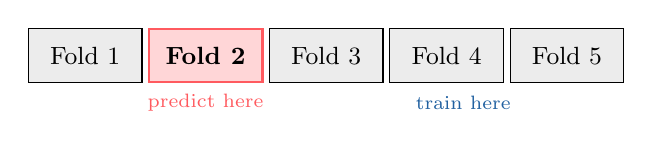
\begin{tikzpicture}[scale=0.85]
\foreach \i in {1,...,5} {
    \draw[fill=gray!15] (\i*1.8-1.8, 0) rectangle (\i*1.8-0.1, 0.8);
    \node at (\i*1.8-0.95, 0.4) {\small Fold \i};
}
% Highlight fold 2
\draw[fill=abnbred!25, draw=abnbred, thick] (1.8, 0) rectangle (3.5, 0.8);
\node at (2.65, 0.4) {\small \textbf{Fold 2}};
\node[font=\scriptsize, abnbred] at (2.65, -0.3) {predict here};
\node[font=\scriptsize, noteblue] at (6.5, -0.3) {train here};
\end{tikzpicture}
\end{center}

For fold $k$: train $\hat{g}^{(-k)}$ (and $\hat{r}^{(-k)}$ if needed) on all folds \emph{except} fold $k$. Compute residuals on fold $k$ using the out-of-sample predictions.

\bigskip

Repeat for all $K$ folds. Stack the residuals.

\bigskip
\pause

Because $\hat{g}^{(-k)}$ never saw observation $i$, it is independent of $(D_i, X_i)$ conditional on the auxiliary sample. This restores the independence Part B needed:
\[
\E\!\left[\tilde{D}_i (g - \hat{g}^{(-k)})(X_i) \;\big|\; \hat{g}^{(-k)}\right] = 0
\]
The overfitting bias vanishes, and the $\sqrt{n}$-averaging argument goes through.

\end{frame}


% ====================================================================
\begin{frame}{Why DML Needs Both Ingredients}

\begin{center}
\begin{tabular}{lcc}
\toprule
\textbf{Problem} & \textbf{Source} & \textbf{Fix} \\
\midrule
Regularization bias & Bias from ML shrinkage; & Orthogonal moment \\
 & first-order in one error & (debiasing/residualization) \\[0.5em]
Overfitting bias & In-sample dependence; & Cross-fitting \\
 & $\hat{g}$ overfits training data & (out-of-sample prediction) \\
\bottomrule
\end{tabular}
\end{center}

\bigskip
\pause

Orthogonality alone is not enough: without cross-fitting, overfitting bias can diverge even at near-parametric rates.

\bigskip

Cross-fitting alone is not enough: without orthogonality, regularization bias diverges at ML rates.

\bigskip

Together: both bias terms vanish, and $\sqrt{n}(\hat{\theta} - \theta_0) \to N(0, V)$.

\end{frame}


% %%%%%%%%%%%%%%%%%%%%%%%%%%%%%%%%%%%%%%%%%%%%%%%%%%%%%%%%%%%%%%%%%%%%
% ACT 2: IMPLEMENTATION (ell/m formulation)
% %%%%%%%%%%%%%%%%%%%%%%%%%%%%%%%%%%%%%%%%%%%%%%%%%%%%%%%%%%%%%%%%%%%%

% %%%%%%%%%%%%%%%%%%%%%%%%%%%%%%%%%%%%%%%%%%%%%%%%%%%%%%%%%%%%%%%%%%%%
\section{From Theory to Practice}
% %%%%%%%%%%%%%%%%%%%%%%%%%%%%%%%%%%%%%%%%%%%%%%%%%%%%%%%%%%%%%%%%%%%%

% ====================================================================
\begin{frame}{From $g$ to $\ell$: What We Actually Estimate}

In practice, we predict $Y$ from $X$ directly:
\[
\ell(X) = \E[Y \mid X] = \theta\, r(X) + g(X)
\]

The residual $Y_i - \ell(X_i)$ removes everything predictable by $X$

\bigskip
\pause

This is the FWL/Robinson approach:

\begin{center}
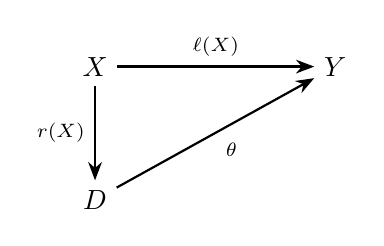
\begin{tikzpicture}[node distance=1.5cm]
\node (X) {$X$};
\node[right=2.5cm of X] (Y) {$Y$};
\node[below=1.2cm of X] (D) {$D$};
\draw[tarrow] (X) -- node[above, font=\scriptsize]{$\ell(X)$} (Y);
\draw[tarrow] (X) -- node[left, font=\scriptsize]{$r(X)$} (D);
\draw[tarrow] (D) -- node[below right, font=\scriptsize]{$\theta$} (Y);
\end{tikzpicture}
\end{center}

Residualize both $D$ and $Y$ against $X$, then regress $\tilde{Y}$ on $\tilde{D}$. DML = FWL with ML.

\end{frame}


% ====================================================================
\begin{frame}{DML Algorithm: Step by Step}

\begin{block}{Double Machine Learning (Chernozhukov et al.\ 2018)}
\begin{enumerate}
    \item \textbf{Split} data into $K$ folds.
    \item \textbf{For each fold $k$:}
    \begin{enumerate}
        \item[(a)] Train $\hat{\ell}^{(-k)}(\cdot)$ on all folds except $k$: predict $Y$ from $X$.
        \item[(b)] Train $\hat{r}^{(-k)}(\cdot)$ on all folds except $k$: predict $D$ from $X$.
        \item[(c)] Compute out-of-sample residuals on fold $k$:
        \[
        \tilde{Y}_i = Y_i - \hat{\ell}^{(-k)}(X_i), \qquad \tilde{D}_i = D_i - \hat{r}^{(-k)}(X_i)
        \]
    \end{enumerate}
    \item \textbf{Stack} all residuals across folds.
    \item \textbf{Regress} $\tilde{Y}$ on $\tilde{D}$ (no intercept). The slope is $\hat{\theta}$.
    \item \textbf{Inference:} standard errors from this regression are valid.
\end{enumerate}
\end{block}

\end{frame}


% ====================================================================
\begin{frame}{What the Residuals Mean}

\begin{center}
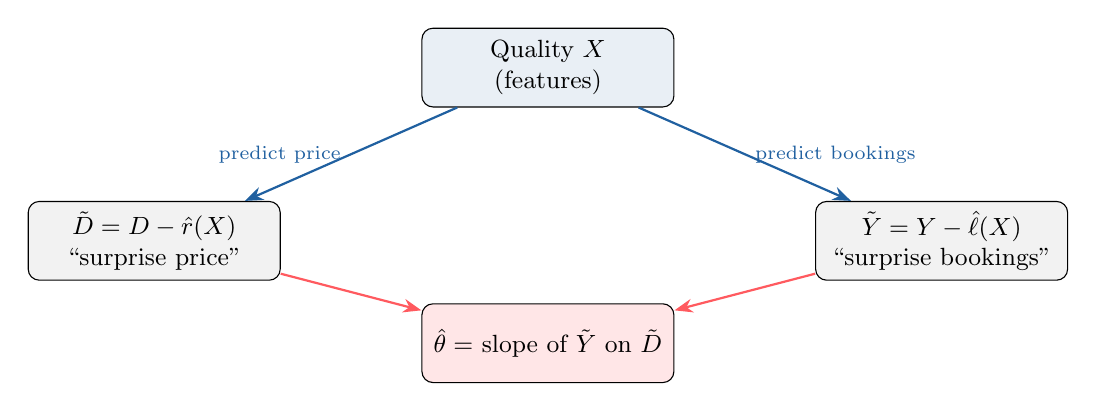
\begin{tikzpicture}[
    block/.style={draw, rounded corners, minimum width=3.2cm, minimum height=1.0cm,
                  font=\small, align=center}
]
\node[block, fill=noteblue!10] (X)     at (5, 2.2)  {Quality $X$\\(features)};
\node[block, fill=gray!10]     (Dtil)  at (0, 0)    {$\tilde{D} = D - \hat{r}(X)$\\``surprise price''};
\node[block, fill=gray!10]     (Ytil)  at (10, 0)   {$\tilde{Y} = Y - \hat{\ell}(X)$\\``surprise bookings''};
\node[block, fill=abnbred!15]  (theta) at (5, -1.3) {$\hat{\theta} = $ slope of $\tilde{Y}$ on $\tilde{D}$};

\draw[tarrow, noteblue] (X) -- node[left, font=\scriptsize]{predict price} (Dtil);
\draw[tarrow, noteblue] (X) -- node[right, font=\scriptsize]{predict bookings} (Ytil);
\draw[tarrow, abnbred, thick]  (Dtil) -- (theta);
\draw[tarrow, abnbred, thick]  (Ytil) -- (theta);
\end{tikzpicture}
\end{center}

$\tilde{D}$: a listing priced higher (or lower) than similar listings.

$\tilde{Y}$: a listing booked more (or less) than similar listings.

$\hat{\theta}$: when $\tilde{D}$ is positive (overpriced), what happens to $\tilde{Y}$ (bookings)?

\end{frame}


% ====================================================================
\begin{frame}{ML Model Choice}

\textbf{For steps 2(a) and 2(b):} any ML model with good out-of-sample prediction.

\bigskip

\begin{center}
\begin{tabular}{ll}
\toprule
\textbf{Model} & \textbf{Notes} \\
\midrule
Random Forest & Good default; handles nonlinearities \\
Gradient Boosting (XGBoost) & Often best prediction accuracy \\
Lasso / Ridge & Works well if nuisance is approximately sparse/linear \\
Neural Network & For complex data (text, images) \\
\bottomrule
\end{tabular}
\end{center}

\bigskip
\pause

The choice of ML model matters for finite-sample performance but not for the asymptotic theory (as long as nuisance estimates converge fast enough).

\bigskip

\textbf{Best practice:} try multiple learners, compare performance, also report sensitivity.

\end{frame}


% ====================================================================
\begin{frame}{What the Residuals Look Like}

After cross-fitting, inspect the residuals before the final regression.

\bigskip

\begin{columns}[T]
\begin{column}{0.48\textwidth}
\textbf{$\tilde{D}$ = price residual}
\begin{itemize}
    \item Mean $\approx 0$
    \item Positive: priced above similar listings
    \item Negative: priced below similar listings
    \item Variation much smaller than raw $D$
\end{itemize}
\end{column}
\begin{column}{0.48\textwidth}
\textbf{$\tilde{Y}$ = bookings residual}
\begin{itemize}
    \item Mean $\approx 0$
    \item Positive: booked more than peers
    \item Negative: booked less than peers
    \item Relationship with $\tilde{D}$ is now clean
\end{itemize}
\end{column}
\end{columns}

\bigskip
\pause

\textbf{Sanity check:} the scatter of $\tilde{Y}$ on $\tilde{D}$ should show a clear negative slope. If not, either the model is misspecified or unconfoundedness is violated.

\end{frame}




% %%%%%%%%%%%%%%%%%%%%%%%%%%%%%%%%%%%%%%%%%%%%%%%%%%%%%%%%%%%%%%%%%%%%
\section{The General Principle: Neyman Orthogonality}
% %%%%%%%%%%%%%%%%%%%%%%%%%%%%%%%%%%%%%%%%%%%%%%%%%%%%%%%%%%%%%%%%%%%%

% ====================================================================
\begin{frame}{Stepping Back: What Did We Just Do?}

For the PLR, we saw:
\begin{itemize}
    \item Naive plugin: use raw $D$ in the moment. Bias is first-order in $\hat{g} - g$.
    \item Debiased plugin: replace $D$ with $\tilde{D}$. Bias becomes second-order.
\end{itemize}

\bigskip
\pause

This is an instance of a general principle. The target parameter $\theta_0$ is defined by a moment condition:
\[
\E[m(W; \theta_0, \eta_0)] = 0
\]

where $\eta_0$ is a nuisance parameter. The plugin estimator solves $\frac{1}{n}\sum_i m(W_i; \hat{\theta}, \hat{\eta}) = 0$.

\bigskip
\pause

The question: how sensitive is $\hat{\theta}$ to errors in $\hat{\eta}$? This depends on the choice of score $m$.

\end{frame}

% ====================================================================
\begin{frame}{The Plugin Expansion}

\textbf{Recall the PLR naive plugin bias} (scaled by $\sqrt n$):
\[
\sqrt{n}(\hat\theta_{\text{naive}} - \theta_0) \;=\; \underbrace{\frac{\frac{1}{\sqrt n}\sum_i D_i \varepsilon_i}{\E[D^2]}}_{\text{CLT term}} \;+\; \underbrace{\frac{1}{\E[D^2]} \cdot \frac{1}{\sqrt n}\sum_i D_i\bigl(g(X_i) - \hat g(X_i)\bigr)}_{(\star)\;=\;\text{first-order impact of }\hat g} \;+\; \text{remainder}
\]

\pause
\bigskip

\textbf{Relabel in general notation.} The PLR score is $m(W;\theta,g) = (Y - g(X) - \theta D)\cdot D$, so
\[
\frac{\partial m}{\partial g}(W; \theta_0, g_0) = -D.
\]
The bias $(\star)$ is exactly
\[
(\star) \;=\; J^{-1} \cdot \frac{1}{\sqrt n}\sum_i \underbrace{\frac{\partial m}{\partial \eta}(W_i; \theta_0, \eta_0)}_{=\,-D_i\text{ in PLR}} \cdot \underbrace{(\hat\eta - \eta_0)(X_i)}_{=\,\hat g - g\text{ in PLR}}
\]
with $J = \E[D^2]$. Same object we already analyzed, written in general symbols.

\end{frame}

% ====================================================================
\begin{frame}{Two Ways $(\star)$ Can Blow Up}

Write $(\star) = J^{-1} \cdot \frac{1}{\sqrt n}\sum_i \xi_i$ with summand
\[
\xi_i \;=\; \frac{\partial m}{\partial \eta}(W_i; \theta_0, \eta_0) \cdot (\hat\eta - \eta_0)(X_i)
\]

For $(\star) \to 0$ via CLT, the $\xi_i$ must be (i) mean zero and (ii) independent of $\hat\eta$.

\pause
\bigskip

\textbf{Centering fails (regularization bias).} If $\E[\xi_i \mid \hat\eta] \neq 0$, then $(\star)$ is $\sqrt n$ times a non-vanishing mean and diverges.

\emph{PLR instance:} with the naive score, $\partial_g m_{\text{naive}} = -D$, so $\E[\xi_i \mid \hat g] = -\E[r(X)(g - \hat g)(X) \mid \hat g]$, nonzero whenever $r(X) = \E[D \mid X] \not\equiv 0$. The score's derivative in $g$ is not orthogonal to nuisance perturbations — this is term (A).

\pause
\bigskip

\textbf{Independence fails (overfitting bias).} If $\hat\eta$ is trained on the same $W_i$ used in the sum, the summands are not i.i.d.\ conditional on $\hat\eta$, and the CLT does not apply.

\emph{PLR instance:} the exact issue that motivated cross-fitting.

\end{frame}

% ====================================================================
\begin{frame}{Neyman Orthogonality}

\begin{block}{Neyman Orthogonality (Chernozhukov et al.\ 2018)}
A score $m(W; \theta, \eta)$ is \textbf{Neyman orthogonal} if:
\[
\frac{\partial}{\partial \lambda} \E\bigl[m(W; \theta_0, \eta_0 + \lambda(\eta - \eta_0))\bigr] \Big|_{\lambda=0} = 0 \quad \forall\, \eta
\]
Small perturbations of the nuisance away from $\eta_0$ do not change the moment condition.
\end{block}

\bigskip
\pause

Neyman orthogonality makes $\frac{\partial}{\partial\eta}m$ mean zero, killing the regularization bias in $(\star)$.

\bigskip

Cross-fitting makes $\hat{\eta} - \eta_0$ independent of $W_i$, killing the overfitting bias in $(\star)$.

\bigskip

Together: $(\star) \to 0$, and inference proceeds as if $\eta_0$ were known.

\end{frame}

% ====================================================================
\begin{frame}{What About the Remainder?}

Orthogonality kills the first-order term $(\star)$. What about the second-order remainder?

\pause

The plugin estimator expands around $(\theta_0, \eta_0)$. The second-order remainder has three pieces:
\[
\underbrace{\tfrac{1}{2}\,\E\!\left[\tfrac{\partial^2 m}{\partial \theta^2}\right](\hat\theta - \theta_0)^2}_{\text{square in }\theta} + \underbrace{\tfrac{1}{2}\,\E\!\left[\tfrac{\partial^2 m}{\partial \eta^2}\right](\hat\eta - \eta_0)^2}_{\text{square in }\eta} + \underbrace{\E\!\left[\tfrac{\partial^2 m}{\partial \theta\,\partial \eta}\right](\hat\theta - \theta_0)(\hat\eta - \eta_0)}_{\text{cross term}}
\]

\pause

\textbf{Each piece is small enough.} With $\hat\theta - \theta_0 = O_p(n^{-1/2})$ and $\hat\eta - \eta_0 = o_p(n^{-1/4})$:
\[
(\hat\theta - \theta_0)^2 = O_p(n^{-1}), \quad (\hat\eta - \eta_0)^2 = o_p(n^{-1/2}), \quad (\hat\theta - \theta_0)(\hat\eta - \eta_0) = o_p(n^{-3/4})
\]
all multiplied by $\sqrt n$ and still $\to 0$.

\end{frame}





\begin{frame}{What About the Remainder?}

Orthogonality kills the first-order term $(\star)$. What about the second-order remainder?

\pause

The plugin estimator expands around $(\theta_0, \eta_0)$. The second-order remainder has three pieces:
\[
\underbrace{\tfrac{1}{2}\,\E\!\left[\tfrac{\partial^2 m}{\partial \theta^2}\right](\hat\theta - \theta_0)^2}_{\text{square in }\theta} + \underbrace{\tfrac{1}{2}\,\E\!\left[\tfrac{\partial^2 m}{\partial \eta^2}\right](\hat\eta - \eta_0)^2}_{\text{square in }\eta} + \underbrace{\E\!\left[\tfrac{\partial^2 m}{\partial \theta\,\partial \eta}\right](\hat\theta - \theta_0)(\hat\eta - \eta_0)}_{\text{cross term}}
\]

\pause
\bigskip

\textbf{Connection to ``From One Error to Two.''} For the partialling-out-$D$ score $m_{\text{P}} = (Y - g - \theta D)\,\tilde D$ with $\eta = (g, r)$:
\[
\partial^2_{gg}\, m_{\text{P}} = 0, \qquad \partial^2_{rr}\, m_{\text{P}} = 0, \qquad \partial^2_{gr}\, m_{\text{P}} = 1
\]
Only the cross term survives, which is exactly $\E[(\hat g - g)(\hat r - r)]$, bounded by $\|\hat g - g\|\cdot\|\hat r - r\| = o_p(n^{-1/2})$ via Cauchy–Schwarz. This is the product-of-two-errors result from ``From One Error to Two.''

\end{frame}


% ====================================================================
\begin{frame}{Verification for PLR: Three Scores}
 
Three candidate scores for $\theta_0$ in $Y = \theta D + g(X) + \varepsilon$:
 
\bigskip
 
\textbf{(1) Naive:} $m_{\text{naive}} = (Y - g(X) - \theta D) \cdot D$, \quad nuisance $\eta = g$.
 
\[
\tfrac{\partial}{\partial\lambda}\E[m_{\text{naive}}(W; \theta_0, g_0 + \lambda\Delta g)]\big|_{\lambda=0} = \E[-\Delta g(X) \cdot D] = -\E[r(X)\Delta g(X)] \;\neq 0
\]
 
whenever $r(X) = \E[D \mid X] \not\equiv 0$. \textbf{Not orthogonal.}
 
\bigskip
\pause
 
\textbf{(2) Partialling out $D$:} $m_{\text{P}} = (Y - g(X) - \theta D) \cdot \tilde D$ with $\tilde D = D - r(X)$, \quad nuisance $\eta = (g, r)$.
 
\[
\tfrac{\partial}{\partial\lambda}\E[m_{\text{P}}]\big|_{\lambda=0}: \quad \underbrace{\E[-\tilde D \cdot \Delta g(X)]}_{=\,0 \text{ since } \E[\tilde D \mid X]=0} \;+\; \underbrace{\E[-\varepsilon \cdot \Delta r(X)]}_{=\,0 \text{ since } \E[\varepsilon \mid X]=0} = 0
\]
 
\textbf{Neyman orthogonal.} Residualizing $D$ alone suffices.
 
\end{frame}
 
% ====================================================================
\begin{frame}{Verification for PLR: Three Scores (cont.)}
 
\textbf{(3) Robinson / partialling out:} $m_{\text{R}} = [(Y - \ell(X)) - \theta(D - r(X))](D - r(X))$, nuisance $\eta = (\ell, r)$.
 
Reparametrize the PLR by subtracting $\E[\cdot \mid X]$ from both sides:
\[
Y - \ell(X) = \theta (D - r(X)) + \varepsilon, \qquad \ell(X) = \E[Y \mid X], \;\; r(X) = \E[D \mid X]
\]
 
\[
\tfrac{\partial}{\partial\lambda}\E[m_{\text{R}}]\big|_{\lambda=0}: \quad \underbrace{\E[-\tilde D \Delta\ell]}_{=\,0} + \underbrace{\E[-\varepsilon\Delta r - \theta_0 \tilde D \Delta r]}_{=\,0 \text{ by } \E[\varepsilon \mid X]=\E[\tilde D \mid X]=0} = 0
\]
 
\textbf{Neyman orthogonal.} No structural $g$ to estimate — regress $Y$ and $D$ separately on $X$, then regress the residuals.
 
\pause
\bigskip
 
\textbf{(2) vs.\ (3).} Both are orthogonal and $\sqrt n$-consistent. Robinson's form is preferred in practice: $\ell$ and $r$ are conditional expectations (standard prediction problems), while $g$ in (2) is a structural parameter defined only given $\theta$.
 
\end{frame}



% %%%%%%%%%%%%%%%%%%%%%%%%%%%%%%%%%%%%%%%%%%%%%%%%%%%%%%%%%%%%%%%%%%%%
\section{The General Principle}
% %%%%%%%%%%%%%%%%%%%%%%%%%%%%%%%%%%%%%%%%%%%%%%%%%%%%%%%%%%%%%%%%%%%%

% ====================================================================
\begin{frame}{Beyond PLR: The DML Blueprint}

The DML idea generalizes beyond the PLR. The recipe is always the same:

\bigskip

\begin{enumerate}
    \item Find a moment condition for $\theta$ that is \textbf{insensitive to small errors in the nuisance} (Neyman orthogonality).
    \item Estimate the nuisance with ML using \textbf{cross-fitting}.
    \item Solve the moment condition for $\theta$.
\end{enumerate}

\bigskip
\pause

\begin{center}
\scriptsize
\begin{tabular}{llcc}
\toprule
\textbf{Target} & \textbf{Setting} & \textbf{Non-orthogonal} & \textbf{Orthogonal} \\
\midrule
Regression coefficient & PLR & Plugin with raw $D$ & Partialling out \\
Average treatment effect & Binary treatment & IPW & AIPW (doubly robust) \\
IV coefficient & Linear IV & Plugin with raw $Z$ & Optimal instrument \\
ATT & Binary treatment & Regression adjustment & AIPW for ATT \\
\bottomrule
\end{tabular}
\end{center}

\bigskip

DML = orthogonal score + cross-fitting. This blueprint works for all of the above.

\end{frame}


% % %%%%%%%%%%%%%%%%%%%%%%%%%%%%%%%%%%%%%%%%%%%%%%%%%%%%%%%%%%%%%%%%%%%%
% \section{Extensions}
% % %%%%%%%%%%%%%%%%%%%%%%%%%%%%%%%%%%%%%%%%%%%%%%%%%%%%%%%%%%%%%%%%%%%%

% % ====================================================================
% \begin{frame}{Extension: Heterogeneous Elasticity}

% The PLR estimates a single $\theta$ (average elasticity). But from L7, we may want $\theta(X)$: listing-specific elasticities.

% \bigskip

% The \textbf{Partially Linear Interactive Regression Model}:
% \[
% Y_i = \theta(X_i) \cdot D_i + g(X_i) + \varepsilon_i
% \]

% \bigskip
% \pause

% Estimated using \texttt{CausalForestDML} from the \texttt{econml} package. This combines:
% \begin{itemize}
%     \item DML residualization (handles confounding and continuous treatment)
%     \item Causal forest (estimates heterogeneous effects)
% \end{itemize}

% \bigskip

% Recall from L7: the original causal forest from L5 requires binary treatment and randomization. \texttt{CausalForestDML} lifts both restrictions by embedding the forest within the DML framework.

% \bigskip

% \textbf{Next lecture (L9):} hands-on lab with \texttt{CausalForestDML}.

% \end{frame}


% ====================================================================
\begin{frame}{Key Takeaways}

\begin{enumerate}
    \item \textbf{The naive plugin fails.} Estimating $g(X)$ with ML and plugging in creates a bias of order $\|\hat{g} - g\|$, too slow for $\sqrt{n}$-inference.

    \pause\bigskip

    \item \textbf{Residualizing $D$ fixes the regularization bias.} Replacing $D$ with $\tilde{D} = D - \hat{r}(X)$ turns the bias into a product of two errors: $\|\hat{g} - g\| \cdot \|\hat{r} - r\|$.

    \pause\bigskip

    \item \textbf{Cross-fitting fixes the overfitting bias.} Out-of-sample prediction ensures that the orthogonality argument holds in finite samples.

    \pause\bigskip

    \item \textbf{Together, $\sqrt{n}$-inference is valid.} Each nuisance needs only $n^{-1/4}$ rate (achievable by ML). Standard errors work as if the nuisances were known.

    \pause\bigskip

    \item \textbf{In practice: predict $Y$ and $D$ from $X$, residualize, regress.} This is FWL with ML and cross-fitting.

\end{enumerate}

\end{frame}

\end{document}